% Created by tikzDevice version 0.12.3 on 2020-08-18 17:15:51
% !TEX encoding = UTF-8 Unicode
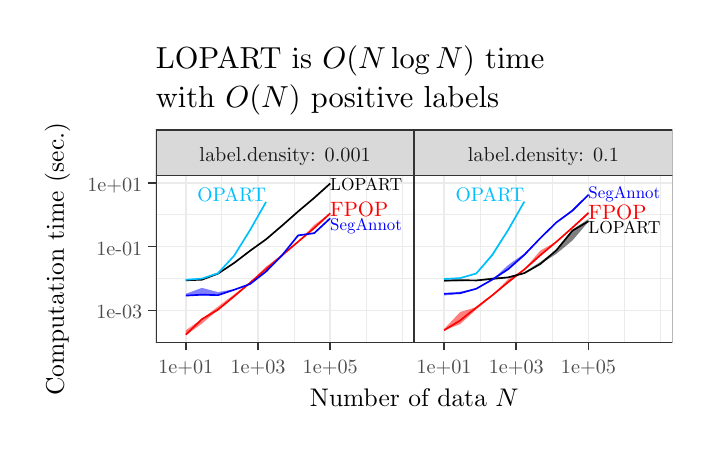
\begin{tikzpicture}[x=1pt,y=1pt]
\definecolor{fillColor}{RGB}{255,255,255}
\path[use as bounding box,fill=fillColor,fill opacity=0.00] (0,0) rectangle (238.49,144.54);
\begin{scope}
\path[clip] (  0.00,  0.00) rectangle (238.49,144.54);
\definecolor{drawColor}{RGB}{255,255,255}
\definecolor{fillColor}{RGB}{255,255,255}

\path[draw=drawColor,line width= 0.6pt,line join=round,line cap=round,fill=fillColor] ( -0.00,  0.00) rectangle (238.49,144.54);
\end{scope}
\begin{scope}
\path[clip] ( 46.36, 30.69) rectangle (139.68, 91.06);
\definecolor{fillColor}{RGB}{255,255,255}

\path[fill=fillColor] ( 46.36, 30.69) rectangle (139.68, 91.06);
\definecolor{drawColor}{gray}{0.92}

\path[draw=drawColor,line width= 0.3pt,line join=round] ( 46.36, 30.89) --
	(139.68, 30.89);

\path[draw=drawColor,line width= 0.3pt,line join=round] ( 46.36, 53.91) --
	(139.68, 53.91);

\path[draw=drawColor,line width= 0.3pt,line join=round] ( 46.36, 76.93) --
	(139.68, 76.93);

\path[draw=drawColor,line width= 0.3pt,line join=round] ( 70.18, 30.69) --
	( 70.18, 91.06);

\path[draw=drawColor,line width= 0.3pt,line join=round] ( 96.28, 30.69) --
	( 96.28, 91.06);

\path[draw=drawColor,line width= 0.3pt,line join=round] (122.39, 30.69) --
	(122.39, 91.06);

\path[draw=drawColor,line width= 0.3pt,line join=round] (135.44, 30.69) --
	(135.44, 91.06);

\path[draw=drawColor,line width= 0.6pt,line join=round] ( 46.36, 42.40) --
	(139.68, 42.40);

\path[draw=drawColor,line width= 0.6pt,line join=round] ( 46.36, 65.42) --
	(139.68, 65.42);

\path[draw=drawColor,line width= 0.6pt,line join=round] ( 46.36, 88.44) --
	(139.68, 88.44);

\path[draw=drawColor,line width= 0.6pt,line join=round] ( 57.13, 30.69) --
	( 57.13, 91.06);

\path[draw=drawColor,line width= 0.6pt,line join=round] ( 83.23, 30.69) --
	( 83.23, 91.06);

\path[draw=drawColor,line width= 0.6pt,line join=round] (109.33, 30.69) --
	(109.33, 91.06);
\definecolor{fillColor}{RGB}{255,0,0}

\path[fill=fillColor,fill opacity=0.50] ( 57.13, 35.20) --
	( 62.97, 39.27) --
	( 68.77, 43.76) --
	( 74.55, 48.08) --
	( 80.34, 52.60) --
	( 86.14, 58.19) --
	( 91.93, 62.51) --
	( 97.73, 67.25) --
	(103.53, 73.26) --
	(109.33, 77.49) --
	(109.33, 77.18) --
	(103.53, 71.99) --
	( 97.73, 67.17) --
	( 91.93, 62.27) --
	( 86.14, 57.23) --
	( 80.34, 52.19) --
	( 74.55, 47.36) --
	( 68.77, 42.56) --
	( 62.97, 37.61) --
	( 57.13, 33.43) --
	cycle;

\path[] ( 57.13, 35.20) --
	( 62.97, 39.27) --
	( 68.77, 43.76) --
	( 74.55, 48.08) --
	( 80.34, 52.60) --
	( 86.14, 58.19) --
	( 91.93, 62.51) --
	( 97.73, 67.25) --
	(103.53, 73.26) --
	(109.33, 77.49);

\path[] (109.33, 77.18) --
	(103.53, 71.99) --
	( 97.73, 67.17) --
	( 91.93, 62.27) --
	( 86.14, 57.23) --
	( 80.34, 52.19) --
	( 74.55, 47.36) --
	( 68.77, 42.56) --
	( 62.97, 37.61) --
	( 57.13, 33.43);
\definecolor{fillColor}{RGB}{0,0,0}

\path[fill=fillColor,fill opacity=0.50] ( 57.13, 53.41) --
	( 62.97, 53.63) --
	( 68.77, 55.85) --
	( 74.55, 59.50) --
	( 80.34, 64.07) --
	( 86.14, 68.06) --
	( 91.93, 73.07) --
	( 97.73, 78.15) --
	(103.53, 83.21) --
	(109.33, 88.31) --
	(109.33, 88.08) --
	(103.53, 82.98) --
	( 97.73, 78.10) --
	( 91.93, 73.00) --
	( 86.14, 68.05) --
	( 80.34, 63.88) --
	( 74.55, 59.44) --
	( 68.77, 55.61) --
	( 62.97, 53.41) --
	( 57.13, 53.23) --
	cycle;

\path[] ( 57.13, 53.41) --
	( 62.97, 53.63) --
	( 68.77, 55.85) --
	( 74.55, 59.50) --
	( 80.34, 64.07) --
	( 86.14, 68.06) --
	( 91.93, 73.07) --
	( 97.73, 78.15) --
	(103.53, 83.21) --
	(109.33, 88.31);

\path[] (109.33, 88.08) --
	(103.53, 82.98) --
	( 97.73, 78.10) --
	( 91.93, 73.00) --
	( 86.14, 68.05) --
	( 80.34, 63.88) --
	( 74.55, 59.44) --
	( 68.77, 55.61) --
	( 62.97, 53.41) --
	( 57.13, 53.23);
\definecolor{fillColor}{RGB}{0,191,255}

\path[fill=fillColor,fill opacity=0.50] ( 57.13, 53.63) --
	( 62.97, 53.94) --
	( 68.77, 56.02) --
	( 74.55, 62.10) --
	( 80.34, 71.40) --
	( 86.14, 81.74) --
	( 86.14, 81.56) --
	( 80.34, 71.31) --
	( 74.55, 62.03) --
	( 68.77, 55.77) --
	( 62.97, 53.57) --
	( 57.13, 53.29) --
	cycle;

\path[] ( 57.13, 53.63) --
	( 62.97, 53.94) --
	( 68.77, 56.02) --
	( 74.55, 62.10) --
	( 80.34, 71.40) --
	( 86.14, 81.74);

\path[] ( 86.14, 81.56) --
	( 80.34, 71.31) --
	( 74.55, 62.03) --
	( 68.77, 55.77) --
	( 62.97, 53.57) --
	( 57.13, 53.29);
\definecolor{fillColor}{RGB}{0,0,255}

\path[fill=fillColor,fill opacity=0.50] ( 57.13, 48.36) --
	( 62.97, 50.51) --
	( 68.77, 48.98) --
	( 74.55, 50.02) --
	( 80.34, 51.89) --
	( 86.14, 56.52) --
	( 91.93, 62.44) --
	( 97.73, 69.66) --
	(103.53, 70.50) --
	(109.33, 75.84) --
	(109.33, 75.56) --
	(103.53, 70.21) --
	( 97.73, 69.38) --
	( 91.93, 62.18) --
	( 86.14, 56.37) --
	( 80.34, 51.83) --
	( 74.55, 49.72) --
	( 68.77, 47.82) --
	( 62.97, 47.84) --
	( 57.13, 47.68) --
	cycle;

\path[] ( 57.13, 48.36) --
	( 62.97, 50.51) --
	( 68.77, 48.98) --
	( 74.55, 50.02) --
	( 80.34, 51.89) --
	( 86.14, 56.52) --
	( 91.93, 62.44) --
	( 97.73, 69.66) --
	(103.53, 70.50) --
	(109.33, 75.84);

\path[] (109.33, 75.56) --
	(103.53, 70.21) --
	( 97.73, 69.38) --
	( 91.93, 62.18) --
	( 86.14, 56.37) --
	( 80.34, 51.83) --
	( 74.55, 49.72) --
	( 68.77, 47.82) --
	( 62.97, 47.84) --
	( 57.13, 47.68);
\definecolor{drawColor}{RGB}{255,0,0}

\path[draw=drawColor,line width= 0.6pt,line join=round] ( 57.13, 33.58) --
	( 62.97, 39.22) --
	( 68.77, 42.63) --
	( 74.55, 47.42) --
	( 80.34, 52.34) --
	( 86.14, 57.30) --
	( 91.93, 62.28) --
	( 97.73, 67.20) --
	(103.53, 72.12) --
	(109.33, 77.46);
\definecolor{drawColor}{RGB}{0,0,0}

\path[draw=drawColor,line width= 0.6pt,line join=round] ( 57.13, 53.26) --
	( 62.97, 53.47) --
	( 68.77, 55.67) --
	( 74.55, 59.47) --
	( 80.34, 63.90) --
	( 86.14, 68.06) --
	( 91.93, 73.01) --
	( 97.73, 78.13) --
	(103.53, 83.02) --
	(109.33, 88.24);
\definecolor{drawColor}{RGB}{0,191,255}

\path[draw=drawColor,line width= 0.6pt,line join=round] ( 57.13, 53.44) --
	( 62.97, 53.87) --
	( 68.77, 55.81) --
	( 74.55, 62.07) --
	( 80.34, 71.37) --
	( 86.14, 81.57);
\definecolor{drawColor}{RGB}{0,0,255}

\path[draw=drawColor,line width= 0.6pt,line join=round] ( 57.13, 47.72) --
	( 62.97, 48.05) --
	( 68.77, 47.88) --
	( 74.55, 49.80) --
	( 80.34, 51.89) --
	( 86.14, 56.42) --
	( 91.93, 62.28) --
	( 97.73, 69.48) --
	(103.53, 70.27) --
	(109.33, 75.66);
\end{scope}
\begin{scope}
\path[clip] ( 46.36, 30.69) rectangle (139.68, 91.06);
\definecolor{drawColor}{RGB}{0,0,255}

\node[text=drawColor,anchor=base west,inner sep=0pt, outer sep=0pt, scale=  0.61] at (109.33, 71.24) {SegAnnot};
\definecolor{drawColor}{RGB}{255,0,0}

\node[text=drawColor,anchor=base west,inner sep=0pt, outer sep=0pt, scale=  0.75] at (109.33, 76.27) {FPOP};
\definecolor{drawColor}{RGB}{0,0,0}

\node[text=drawColor,anchor=base west,inner sep=0pt, outer sep=0pt, scale=  0.63] at (109.33, 85.65) {LOPART};
\definecolor{drawColor}{RGB}{0,191,255}

\node[text=drawColor,anchor=base east,inner sep=0pt, outer sep=0pt, scale=  0.71] at ( 86.14, 81.57) {OPART};
\definecolor{drawColor}{gray}{0.20}

\path[draw=drawColor,line width= 0.6pt,line join=round,line cap=round] ( 46.36, 30.69) rectangle (139.68, 91.06);
\end{scope}
\begin{scope}
\path[clip] (139.68, 30.69) rectangle (232.99, 91.06);
\definecolor{fillColor}{RGB}{255,255,255}

\path[fill=fillColor] (139.68, 30.69) rectangle (232.99, 91.06);
\definecolor{drawColor}{gray}{0.92}

\path[draw=drawColor,line width= 0.3pt,line join=round] (139.68, 30.89) --
	(232.99, 30.89);

\path[draw=drawColor,line width= 0.3pt,line join=round] (139.68, 53.91) --
	(232.99, 53.91);

\path[draw=drawColor,line width= 0.3pt,line join=round] (139.68, 76.93) --
	(232.99, 76.93);

\path[draw=drawColor,line width= 0.3pt,line join=round] (163.50, 30.69) --
	(163.50, 91.06);

\path[draw=drawColor,line width= 0.3pt,line join=round] (189.60, 30.69) --
	(189.60, 91.06);

\path[draw=drawColor,line width= 0.3pt,line join=round] (215.70, 30.69) --
	(215.70, 91.06);

\path[draw=drawColor,line width= 0.3pt,line join=round] (228.75, 30.69) --
	(228.75, 91.06);

\path[draw=drawColor,line width= 0.6pt,line join=round] (139.68, 42.40) --
	(232.99, 42.40);

\path[draw=drawColor,line width= 0.6pt,line join=round] (139.68, 65.42) --
	(232.99, 65.42);

\path[draw=drawColor,line width= 0.6pt,line join=round] (139.68, 88.44) --
	(232.99, 88.44);

\path[draw=drawColor,line width= 0.6pt,line join=round] (150.44, 30.69) --
	(150.44, 91.06);

\path[draw=drawColor,line width= 0.6pt,line join=round] (176.55, 30.69) --
	(176.55, 91.06);

\path[draw=drawColor,line width= 0.6pt,line join=round] (202.65, 30.69) --
	(202.65, 91.06);
\definecolor{fillColor}{RGB}{255,0,0}

\path[fill=fillColor,fill opacity=0.50] (150.44, 35.61) --
	(156.28, 41.78) --
	(162.09, 43.55) --
	(167.86, 47.93) --
	(173.65, 53.65) --
	(179.45, 57.32) --
	(185.25, 63.96) --
	(191.05, 67.27) --
	(196.85, 72.42) --
	(202.65, 78.03) --
	(202.65, 77.28) --
	(196.85, 72.12) --
	(191.05, 67.11) --
	(185.25, 62.17) --
	(179.45, 57.12) --
	(173.65, 52.38) --
	(167.86, 47.48) --
	(162.09, 42.73) --
	(156.28, 37.44) --
	(150.44, 35.13) --
	cycle;

\path[] (150.44, 35.61) --
	(156.28, 41.78) --
	(162.09, 43.55) --
	(167.86, 47.93) --
	(173.65, 53.65) --
	(179.45, 57.32) --
	(185.25, 63.96) --
	(191.05, 67.27) --
	(196.85, 72.42) --
	(202.65, 78.03);

\path[] (202.65, 77.28) --
	(196.85, 72.12) --
	(191.05, 67.11) --
	(185.25, 62.17) --
	(179.45, 57.12) --
	(173.65, 52.38) --
	(167.86, 47.48) --
	(162.09, 42.73) --
	(156.28, 37.44) --
	(150.44, 35.13);
\definecolor{fillColor}{RGB}{0,0,0}

\path[fill=fillColor,fill opacity=0.50] (150.44, 53.27) --
	(156.28, 53.33) --
	(162.09, 53.36) --
	(167.86, 54.22) --
	(173.65, 54.52) --
	(179.45, 56.16) --
	(185.25, 59.88) --
	(191.05, 64.14) --
	(196.85, 71.49) --
	(202.65, 75.41) --
	(202.65, 74.43) --
	(196.85, 67.64) --
	(191.05, 62.82) --
	(185.25, 59.10) --
	(179.45, 55.64) --
	(173.65, 54.24) --
	(167.86, 53.58) --
	(162.09, 53.19) --
	(156.28, 52.94) --
	(150.44, 52.74) --
	cycle;

\path[] (150.44, 53.27) --
	(156.28, 53.33) --
	(162.09, 53.36) --
	(167.86, 54.22) --
	(173.65, 54.52) --
	(179.45, 56.16) --
	(185.25, 59.88) --
	(191.05, 64.14) --
	(196.85, 71.49) --
	(202.65, 75.41);

\path[] (202.65, 74.43) --
	(196.85, 67.64) --
	(191.05, 62.82) --
	(185.25, 59.10) --
	(179.45, 55.64) --
	(173.65, 54.24) --
	(167.86, 53.58) --
	(162.09, 53.19) --
	(156.28, 52.94) --
	(150.44, 52.74);
\definecolor{fillColor}{RGB}{0,191,255}

\path[fill=fillColor,fill opacity=0.50] (150.44, 54.01) --
	(156.28, 54.07) --
	(162.09, 55.78) --
	(167.86, 63.01) --
	(173.65, 71.79) --
	(179.45, 81.81) --
	(179.45, 81.39) --
	(173.65, 71.42) --
	(167.86, 62.08) --
	(162.09, 55.67) --
	(156.28, 53.95) --
	(150.44, 53.48) --
	cycle;

\path[] (150.44, 54.01) --
	(156.28, 54.07) --
	(162.09, 55.78) --
	(167.86, 63.01) --
	(173.65, 71.79) --
	(179.45, 81.81);

\path[] (179.45, 81.39) --
	(173.65, 71.42) --
	(167.86, 62.08) --
	(162.09, 55.67) --
	(156.28, 53.95) --
	(150.44, 53.48);
\definecolor{fillColor}{RGB}{0,0,255}

\path[fill=fillColor,fill opacity=0.50] (150.44, 48.43) --
	(156.28, 49.14) --
	(162.09, 50.29) --
	(167.86, 53.51) --
	(173.65, 58.76) --
	(179.45, 62.88) --
	(185.25, 68.62) --
	(191.05, 74.24) --
	(196.85, 78.89) --
	(202.65, 84.28) --
	(202.65, 84.14) --
	(196.85, 78.39) --
	(191.05, 74.04) --
	(185.25, 68.23) --
	(179.45, 62.41) --
	(173.65, 57.24) --
	(167.86, 53.39) --
	(162.09, 50.14) --
	(156.28, 48.40) --
	(150.44, 47.76) --
	cycle;

\path[] (150.44, 48.43) --
	(156.28, 49.14) --
	(162.09, 50.29) --
	(167.86, 53.51) --
	(173.65, 58.76) --
	(179.45, 62.88) --
	(185.25, 68.62) --
	(191.05, 74.24) --
	(196.85, 78.89) --
	(202.65, 84.28);

\path[] (202.65, 84.14) --
	(196.85, 78.39) --
	(191.05, 74.04) --
	(185.25, 68.23) --
	(179.45, 62.41) --
	(173.65, 57.24) --
	(167.86, 53.39) --
	(162.09, 50.14) --
	(156.28, 48.40) --
	(150.44, 47.76);
\definecolor{drawColor}{RGB}{255,0,0}

\path[draw=drawColor,line width= 0.6pt,line join=round] (150.44, 35.17) --
	(156.28, 38.74) --
	(162.09, 43.38) --
	(167.86, 47.82) --
	(173.65, 52.61) --
	(179.45, 57.16) --
	(185.25, 62.31) --
	(191.05, 67.16) --
	(196.85, 72.29) --
	(202.65, 77.58);
\definecolor{drawColor}{RGB}{0,0,0}

\path[draw=drawColor,line width= 0.6pt,line join=round] (150.44, 53.19) --
	(156.28, 53.30) --
	(162.09, 53.20) --
	(167.86, 53.76) --
	(173.65, 54.30) --
	(179.45, 55.83) --
	(185.25, 59.14) --
	(191.05, 64.12) --
	(196.85, 71.19) --
	(202.65, 74.58);
\definecolor{drawColor}{RGB}{0,191,255}

\path[draw=drawColor,line width= 0.6pt,line join=round] (150.44, 53.74) --
	(156.28, 54.05) --
	(162.09, 55.71) --
	(167.86, 62.35) --
	(173.65, 71.49) --
	(179.45, 81.67);
\definecolor{drawColor}{RGB}{0,0,255}

\path[draw=drawColor,line width= 0.6pt,line join=round] (150.44, 48.40) --
	(156.28, 48.59) --
	(162.09, 50.20) --
	(167.86, 53.49) --
	(173.65, 57.28) --
	(179.45, 62.42) --
	(185.25, 68.50) --
	(191.05, 74.17) --
	(196.85, 78.41) --
	(202.65, 84.18);
\end{scope}
\begin{scope}
\path[clip] (139.68, 30.69) rectangle (232.99, 91.06);
\definecolor{drawColor}{RGB}{0,0,0}

\node[text=drawColor,anchor=base west,inner sep=0pt, outer sep=0pt, scale=  0.63] at (202.65, 70.05) {LOPART};
\definecolor{drawColor}{RGB}{255,0,0}

\node[text=drawColor,anchor=base west,inner sep=0pt, outer sep=0pt, scale=  0.75] at (202.65, 75.23) {FPOP};
\definecolor{drawColor}{RGB}{0,0,255}

\node[text=drawColor,anchor=base west,inner sep=0pt, outer sep=0pt, scale=  0.61] at (202.65, 82.85) {SegAnnot};
\definecolor{drawColor}{RGB}{0,191,255}

\node[text=drawColor,anchor=base east,inner sep=0pt, outer sep=0pt, scale=  0.71] at (179.45, 81.67) {OPART};
\definecolor{drawColor}{gray}{0.20}

\path[draw=drawColor,line width= 0.6pt,line join=round,line cap=round] (139.68, 30.69) rectangle (232.99, 91.06);
\end{scope}
\begin{scope}
\path[clip] ( 46.36, 91.06) rectangle (139.68,107.63);
\definecolor{drawColor}{gray}{0.20}
\definecolor{fillColor}{gray}{0.85}

\path[draw=drawColor,line width= 0.6pt,line join=round,line cap=round,fill=fillColor] ( 46.36, 91.06) rectangle (139.68,107.63);
\definecolor{drawColor}{gray}{0.10}

\node[text=drawColor,anchor=base,inner sep=0pt, outer sep=0pt, scale=  0.73] at ( 93.02, 96.31) {label.density: 0.001};
\end{scope}
\begin{scope}
\path[clip] (139.68, 91.06) rectangle (232.99,107.63);
\definecolor{drawColor}{gray}{0.20}
\definecolor{fillColor}{gray}{0.85}

\path[draw=drawColor,line width= 0.6pt,line join=round,line cap=round,fill=fillColor] (139.68, 91.06) rectangle (232.99,107.63);
\definecolor{drawColor}{gray}{0.10}

\node[text=drawColor,anchor=base,inner sep=0pt, outer sep=0pt, scale=  0.73] at (186.33, 96.31) {label.density: 0.1};
\end{scope}
\begin{scope}
\path[clip] (  0.00,  0.00) rectangle (238.49,144.54);
\definecolor{drawColor}{gray}{0.20}

\path[draw=drawColor,line width= 0.6pt,line join=round] ( 57.13, 27.94) --
	( 57.13, 30.69);

\path[draw=drawColor,line width= 0.6pt,line join=round] ( 83.23, 27.94) --
	( 83.23, 30.69);

\path[draw=drawColor,line width= 0.6pt,line join=round] (109.33, 27.94) --
	(109.33, 30.69);
\end{scope}
\begin{scope}
\path[clip] (  0.00,  0.00) rectangle (238.49,144.54);
\definecolor{drawColor}{gray}{0.30}

\node[text=drawColor,anchor=base,inner sep=0pt, outer sep=0pt, scale=  0.73] at ( 57.13, 19.68) {1e+01};

\node[text=drawColor,anchor=base,inner sep=0pt, outer sep=0pt, scale=  0.73] at ( 83.23, 19.68) {1e+03};

\node[text=drawColor,anchor=base,inner sep=0pt, outer sep=0pt, scale=  0.73] at (109.33, 19.68) {1e+05};
\end{scope}
\begin{scope}
\path[clip] (  0.00,  0.00) rectangle (238.49,144.54);
\definecolor{drawColor}{gray}{0.20}

\path[draw=drawColor,line width= 0.6pt,line join=round] (150.44, 27.94) --
	(150.44, 30.69);

\path[draw=drawColor,line width= 0.6pt,line join=round] (176.55, 27.94) --
	(176.55, 30.69);

\path[draw=drawColor,line width= 0.6pt,line join=round] (202.65, 27.94) --
	(202.65, 30.69);
\end{scope}
\begin{scope}
\path[clip] (  0.00,  0.00) rectangle (238.49,144.54);
\definecolor{drawColor}{gray}{0.30}

\node[text=drawColor,anchor=base,inner sep=0pt, outer sep=0pt, scale=  0.73] at (150.44, 19.68) {1e+01};

\node[text=drawColor,anchor=base,inner sep=0pt, outer sep=0pt, scale=  0.73] at (176.55, 19.68) {1e+03};

\node[text=drawColor,anchor=base,inner sep=0pt, outer sep=0pt, scale=  0.73] at (202.65, 19.68) {1e+05};
\end{scope}
\begin{scope}
\path[clip] (  0.00,  0.00) rectangle (238.49,144.54);
\definecolor{drawColor}{gray}{0.30}

\node[text=drawColor,anchor=base east,inner sep=0pt, outer sep=0pt, scale=  0.73] at ( 41.41, 39.37) {1e-03};

\node[text=drawColor,anchor=base east,inner sep=0pt, outer sep=0pt, scale=  0.73] at ( 41.41, 62.39) {1e-01};

\node[text=drawColor,anchor=base east,inner sep=0pt, outer sep=0pt, scale=  0.73] at ( 41.41, 85.41) {1e+01};
\end{scope}
\begin{scope}
\path[clip] (  0.00,  0.00) rectangle (238.49,144.54);
\definecolor{drawColor}{gray}{0.20}

\path[draw=drawColor,line width= 0.6pt,line join=round] ( 43.61, 42.40) --
	( 46.36, 42.40);

\path[draw=drawColor,line width= 0.6pt,line join=round] ( 43.61, 65.42) --
	( 46.36, 65.42);

\path[draw=drawColor,line width= 0.6pt,line join=round] ( 43.61, 88.44) --
	( 46.36, 88.44);
\end{scope}
\begin{scope}
\path[clip] (  0.00,  0.00) rectangle (238.49,144.54);
\definecolor{drawColor}{RGB}{0,0,0}

\node[text=drawColor,anchor=base,inner sep=0pt, outer sep=0pt, scale=  0.92] at (139.68,  7.64) {Number of data $N$};
\end{scope}
\begin{scope}
\path[clip] (  0.00,  0.00) rectangle (238.49,144.54);
\definecolor{drawColor}{RGB}{0,0,0}

\node[text=drawColor,rotate= 90.00,anchor=base,inner sep=0pt, outer sep=0pt, scale=  0.92] at ( 13.08, 60.87) {Computation time (sec.)};
\end{scope}
\begin{scope}
\path[clip] (  0.00,  0.00) rectangle (238.49,144.54);
\definecolor{drawColor}{RGB}{0,0,0}

\node[text=drawColor,anchor=base west,inner sep=0pt, outer sep=0pt, scale=  1.10] at ( 46.36,129.95) {LOPART is $O(N\log N)$ time};

\node[text=drawColor,anchor=base west,inner sep=0pt, outer sep=0pt, scale=  1.10] at ( 46.36,115.69) {with $O(N)$ positive labels};
\end{scope}
\end{tikzpicture}
